\section{Auswertung}
\label{sec:Auswertung}
    In Tabelle \ref{tab:Messdaten} sind beide gemessenen Temperaturen, 
    Drücke sowie die Arbeit in Abhängigkeit der Zeit aufgetragen.
    Die Messunsicherheiten betragen $\pm 0.1\,°C$ für beide Temperaturen,
    $\pm 0.5\,°C$ für beide Drücke sowie $\pm 5$\, Watt für die Arbeit.
    \begin{table}[H]
      \centering
      \label{tab:Messdaten}
      \caption{Die Messwerte beider Drücke, der Temperaturen beider Reservoirs sowie 
      die Arbeit zu verschiedenen Zeiten.}
      \begin{tblr}{colspec={c c c c c c}}
      \toprule
      $t$ / min & $T_\text{b}$ / °C & $p_\text{b}$ / bar &
      $T_\text{a}$ / °C & $p_\text{a}$ / bar & $A$ / W\\ 
      \midrule
      1  & 21,5 & 4,4  &  21,0 & 4,1 & 150\\
      2  & 22,0 & 6,0  &  21,0 & 1,4 & 165\\
      3  & 22,8 & 6,2  &  21,0 & 1,6 & 175\\
      4  & 23,8 & 6,6  &  20,4 & 2,0 & 185\\
      5  & 26,7 & 7,5  &  17,4 & 2,1 & 200\\
      6  & 28,5 & 8,0  &  15,6 & 2,2 & 200\\
      7  & 30,3 & 8,2  &  13,9 & 2,2 & 200\\
      8  & 32,0 & 8,6  &  12,2 & 2,2 & 205\\
      9  & 33,7 & 9,0  &  10,6 & 2,2 & 205\\
      10 & 35,4 & 9,4  &  9,0  & 2,2 & 206\\
      11 & 37,0 & 9,7  &  7,5  & 2,2 & 210\\
      12 & 38,5 & 10,1 &  6,2 & 2,3 & 210\\
      13 & 40,1 & 10,4 &  5,1 & 2,3 & 210\\
      14 & 41,6 & 10,8 &  4,1 & 2,3 & 210\\
      15 & 43,0 & 11,0 &  3,4 & 2,3 & 210\\
      16 & 44,4 & 11,5 &  2,8 & 2,3 & 210\\
      17 & 45,6 & 11,7 &  2,2 & 2,3 & 210\\
      18 & 46,8 & 12,0 &  1,7 & 2,3 & 210\\
      19 & 48,0 & 12,2 &  1,3 & 2,3 & 210\\
      20 & 49,0 & 12,5 &  0,9 & 2,2 & 205\\
      21 & 50,0 & 12,8 &  0,4 & 2,2 & 205\\
      \bottomrule
      \end{tblr}
    \end{table}
    \begin{figure}
        \centering
        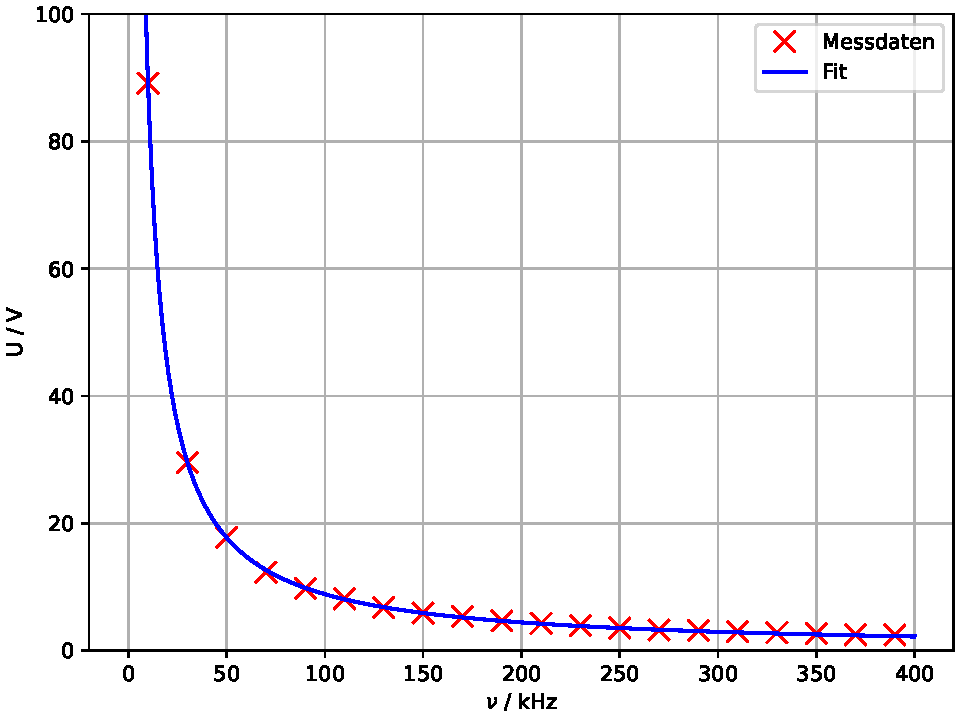
\includegraphics[height= 5cm]{build/plota.pdf}
        \caption{Die Temperatur in Abhängigkeit der Zeit der beiden Reservoire.}
        \label{fig:Fit_Temperatur}
    \end{figure}
    \subsection{Ausgleichsrechnung}
    Abbildung \ref{fig:Fit_Temperatur} zeigt die Messwerte der Messreihen für $T_1$
    und $T_2$ sowie die Plots einer nichtlinearen Ausgleichsrechnung der Messwerte.
    Für die Ausgleichsrechnung werde die Funktion
    \begin{equation}
        T(t) = at^2+bt+c
        \label{eq:Ausgleich}
    \end{equation}
    gewählt.
    Mittels Python werden folgende Werte errechnet
    \begin{align*}
        a_1 &= \SI{-4.6(1.1)e-6}{\degreeCelsius\per\square\second}
        & a_2 &= \SI{10.4(1.9)e-6}{\degreeCelsius\per\square\second}\\
        b_1 &= \SI{3.2(0.2)e-2}{\degreeCelsius\per\second}
        & b_2 &=\SI{3.3(0.3)e-2}{\degreeCelsius\per\second}\\
        c_1 &=\SI{18.0(0.4)}{\degreeCelsius}
        & c_2 &=\SI{25.6(0.7)}{\degreeCelsius}
    \end{align*}
    wobei die Werte mit dem Index 1 den Verlauf der blauen Kurve beschreiben
    und die Werte mit dem Index 2 den der orangenen Kurve beschreiben.

    \subsection{Berechnung der Differentialquotienten}
    Die Differentialquotienen $\sfrac{\text{d}T_i}{\text{d}t}$ berechnen sich durch einsetzen von $t$ in die Ableitung
    von Gl. \eqref{eq:Ausgleich}, $T'(t) = 2at+b$\,.
    Die errechneten Werte der Ableitung sind in \autoref{tab:Diffquot} dargestellt.
    \begin{table}[H]
      \centering
      \begin{tabular}{
        S[table-format=4.0]
        S[table-format=2.3]
        S[table-format=2.3]
        S[table-format=3.0]
      }
        \toprule
        {$t\left[\unit{s}\right]$} & {$\frac{\text{d}T_1}{\text{d}t}\left[\unit{\frac{°C}{s}}\right]$}
        & {$\frac{\text{d}T_2}{\text{d}t}\left[\unit{\frac{°C}{s}}\right]$} & {$N\,\left[\unit{W}\right]$}\\
        \midrule
        300 &  {$0,029 \pm 0,002$}  & {$-0,027 \pm 0,004$} & 200\\
        600 &  {$0,026 \pm 0,003$}  & {$-0,021 \pm 0,005$} & 206\\
        900 &  {$0,023 \pm 0,004$}  & {$-0,015 \pm 0,006$} & 210\\
        1200 & {$0,021 \pm 0,004$}  & {$-0,008 \pm 0,007$} & 205\\
        \bottomrule
    \end{tabular}
      \label{tab:Diffquot}
    \caption{Differentialquotienten für vier Zeiten der zwei Messreihen. Mhhh sind das echt zwei Messreihen?
    Weil basically ist es ja eine Messreihe gewesen, wie kann man das maybe noch anders ausdrücken?}
    \end{table}

    \subsection{Berechnung der Güteziffer}
    Die ideale Güterziffer lässt sich über ??? berechnen.
    Die reale Güteziffer wird mit ??? berechnent.
    Hierbei gilt $m_1 = 3\,\unit{kg}$ und $c_w = \SI{4200}{\joule\per\kg\per\kelvin}$.
    Die Wärmekapazität der Kupferschlange und der Reservoire ist $m_\text{k} c_\text{k} = \SI{750}{\joule\per\kelvin}$.
    Die Güteziffern sind in \autoref{tab:Guete} aufgeführt.
    \begin{table}
  \centering
  \begin{tabular}{
    S[table-format=4.0]
    S[table-format=2.3]
    S[table-format=2.3]
    S[table-format=2.3]
    S[table-format=2.3]
    S[table-format=2.3]
  }
    \toprule
    {$t\left[\unit{s}\right]$} & {$v_{\text{ideal}}$} & {$v_{\text{real}}$ für $T_1$} & {$v_{\text{real}}$ für $T_2$}
    & {$\Delta v_1$} & {$\Delta v_2$}\\
    \midrule
    300 & 2.87  & {$1,9 \pm 0,1$} & {$-1,8 \pm 0,3$} & 0.94 & 1.07\\
    600 & 1.34  & {$1,7 \pm 0,2$} & {$-1,4 \pm 0,3$} & 0.34 & 0.02\\
    900 & 1.09  & {$1,5 \pm 0,3$} & {$-1,0 \pm 0,4$} & 0.37 & 0.14\\
    1200 & 1.02 & {$1,4 \pm 0,3$} & {$-0,5 \pm 0,5$} & 0.35 & 0.50\\
    \bottomrule
\end{tabular}
\caption{Ideale und reale Güteziffer für vier Zeiten und deren Abweichung}
        \label{tab:Guete}
\end{table}

    \subsection{Die Verdampfungswärme L}
    Die Verdampfungswärme des Transportgases kann aus seiner Dampfdruckkurve bestimmt werden.
    Die Dampfdruck-Kurve wird aus den Messwerten $T_1$ und $p_\text{b}$ gewonnen.
    Dafür wird der Logarithmus der Drucks $p_\text{b}$ gegen die reziproke absolute Temperatur $T_1$ aufgetragen.
    \begin{figure}[H]
        \centering
        \includegraphics[height=7cm]{build/Verdampfungswärme.pdf}
        \caption{Die Messwerte des warmen Reservoirs aufgetragen als
        der Logarithmus der Drucks $p_\text{b}$ gegen die reziproke absolute Temperatur
        $T_1$ mit der Ausgleichsgeraden. $p_0 = \qty{1001}{\milli\bar}$}
    \end{figure}
    Die Gleichung zur Bestimmung von $L$ und dem damit einhergehenden Fit ist
    \begin{equation}
        \ln(p) = - \frac{L}{R} \cdot \frac{1}{T}
        \Rightarrow y = m \cdot x + b \, \text{.}
    \end{equation}
    Nummeric Python berechnet $m = \SI{2726 \pm 179}{\kelvin}$ und $b = 4.1 \pm 0.6$.
    Damit ergibt sich mit $L = -a \cdot R$, wobei $R$ die Universelle Gaskonstante mit dem Wert
    $R = \SI{8.314}{\joule\per\mole\per\kelvin}$ \cite{Gaskonstante},
    \begin{equation*}
        L = \SI{2.27(0.15)e+4}{\joule\per\mol} \, \text{.}
    \end{equation*}
\subsection{Bestimmung der mechanischen Arbeit}
Der Sinn einer Wärmepumpe ist, im idealen Falle nur die Arbeit
zur Phasenumwandlung aufzuwenden. Diese mechanisch geleistete Arbeit soll nun berechnet
werden. Um die dazu in der Theorie angegebene Gl. \eqref{eq:mechanisch} anwenden zu können,
muss zunächst $\rho$ bestimmt werden. Dazu wird die allgemeine Gasgleichung verwendet
\begin{equation}
  pV=n\text{R}T\,.
\end{equation}
Es gilt $n\text{R}=\text{const.}$, woraus folgt dass $n_1\text{R}=n_2\text{R}$ korrekt ist.
Über dies und die Beziehung $V=\sfrac{m}{\rho}$ lässt sich für $\rho$ herleiten, dass
\begin{equation}
  \frac{p_0V_0}{T_0}=\frac{p_2V_2}{T_2}\Leftrightarrow
  \frac{p_0}{\rho_0T_0}=\frac{p_\text{a}}{T_2\rho}\Leftrightarrow
  \rho=\frac{\rho_0T_0p_\text{a}}{T_2p_0}\,.
\end{equation}